\documentclass[fleqn,reqno,10pt]{article}

%========================================
% Packages
%========================================

\usepackage[]{latex-helpers/mypackages}
%\usepackage[natbib=true,style=authoryear-comp,backend=bibtex,doi=false,url=false]{biblatex}
\bibliography{project-bib.bib}
\usepackage{latex-helpers/myenvironments}
\usepackage{latex-helpers/mycommands}



%========================================
% Standard Layout
%========================================

% Itemize
\renewcommand{\labelitemi}{\large{$\mathbf{\cdot}$}}    % itemize symbols
\renewcommand{\labelitemii}{\large{$\mathbf{\cdot}$}}
\renewcommand{\labelitemiii}{\large{$\mathbf{\cdot}$}}
\renewcommand{\labelitemiv}{\large{$\mathbf{\cdot}$}}
% Description
\renewcommand{\descriptionlabel}[1]{\hspace\labelsep\textsc{#1}}

% Figure Captions
\usepackage{caption} % use corresponding myfiguresize!
\setlength{\captionmargin}{20pt}
\renewcommand{\captionfont}{\small}
\setlength{\belowcaptionskip}{7pt} % standard is 0pt


\title{Inferences from Causal Attribution}
\author{Tadeg Quillien \& Michael Franke}
\date{}

\begin{document}
\maketitle



\section{Study 1}

We study whether people infer the prescriptive norm a speaker holds, based on a causal judgment made by the speaker. 

\citet{kirfel2022inference} found preliminary evidence for such an ability: they found that listeners make systematic inferences about a prescriptive norm (whether a worker is allowed to show up at work at a particular time) from a speaker's causal judgment. In the vignette they use, two workers show up at work one morning, but only one of them was allowed to be there. Their presence activates a motion detector. 

Kirfel et al. find that when the speaker says `Billy caused the motion detector to activate', listeners infer that Billy wasn't allowed to come to work in the condition where the causal structure is conjunctive, and infer that the other worker wasn't allowed to come to work in the condition where the structure is disjunctive. This is the pattern of effects one expects if listeners are reverse-engineering the counterfactual simulation process involved in causal judgment, as articulated in recent computational models
\citep{icard2017normality, quillien2020when, quillien2023counterfactuals}


However, that preliminary study has an important limitation, because prescriptive normality is confounded with statistical normality: if someone is ordered to stay at home, it is surprising (i.e. statistically unlikely) for that person to show up to work. Since statistical normality also impacts causal judgment, it is unknown whether the effect found by Kirfel et al. is explained by an inference of prescriptive or statistical normality.

Additionally, Kirfel et al. asked participants to make causal judgments themselves before they had to make inferences from the causal judgments of other speakers. As such we don't know to what extent listeners can make these inferences spontaneously.

We designed Study 1 to address these two points. Additionally, we manipulate the valence of the outcome, to see if listeners also use this information to derive inferences.

\subsection{Methods}
In order to manipulate prescriptive normality independently of statistical normality, we designed a story in which the prescriptive norm cannot influence the probability of an outcome. Specifically, the agent in our story interacts with a `marble machine' which can release marbles of different colors; which colors are released is stochastic and completely outside of the agent's control. The agent holds a moral preference regarding which color should be released, but this preference cannot impact which color actually is released. Depending on the combination of colors released by the machine, one of two sounds (A and B) is played. The rule that determines which sound plays as a function of the colors is common knowledge.

Participants see another agent (henceforth, the `speaker') use the machine, releasing a blue and a red marble, which triggers sound A. The speaker makes a causal judgment, selecting one of the marbles as having caused sound A to be played. Participants are asked to infer the prescriptive norm held by the speaker, i.e. whether the speaker thinks red marbles or blue marbles should not be released. We manipulate:
\begin{itemize}
\item The causal structure determining whether sound A plays: either conjunctive (sound A plays if a red marble AND a blue marble get released) or disjunctive (sound A plays if a red marble OR a blue marble get released).

\item The valence of the outcome: sound A is either pleasant (`a pleasant melody'), neutral (`a simple tone') or unpleasant (`a distressing, screeching noise'). Sound B (the sound that did not get played) is always `a simple tone'.

\end{itemize}


Our experiment is thus a 2 (structure) * 3 (valence) between-subjects design.

\subsubsection{Procedure}

We told participants a story about inhabitants of an island who, long ago, discovered an artifact of unknown origin called the `marble machine'. The machine has two compartments; the left compartment contains blue and yellow marbles in equal proportions, while the right compartment contains red and green marbles in equal proportions, see Figure \ref{fig:sub1}. When a user presses the `start' button, one marble is randomly released from each compartment. Depending on the colors of the two marbles that get released, the machine plays a sound, either A or B. In the \textbf{conjunctive} structure condition, sound A plays if both a blue marble and a red marble are released. In the \textbf{disjunctive} structure condition, sound A plays if either a blue marble or a red marble is released.

\begin{figure*}
\begin{subfigure}{.5\textwidth}
\centering
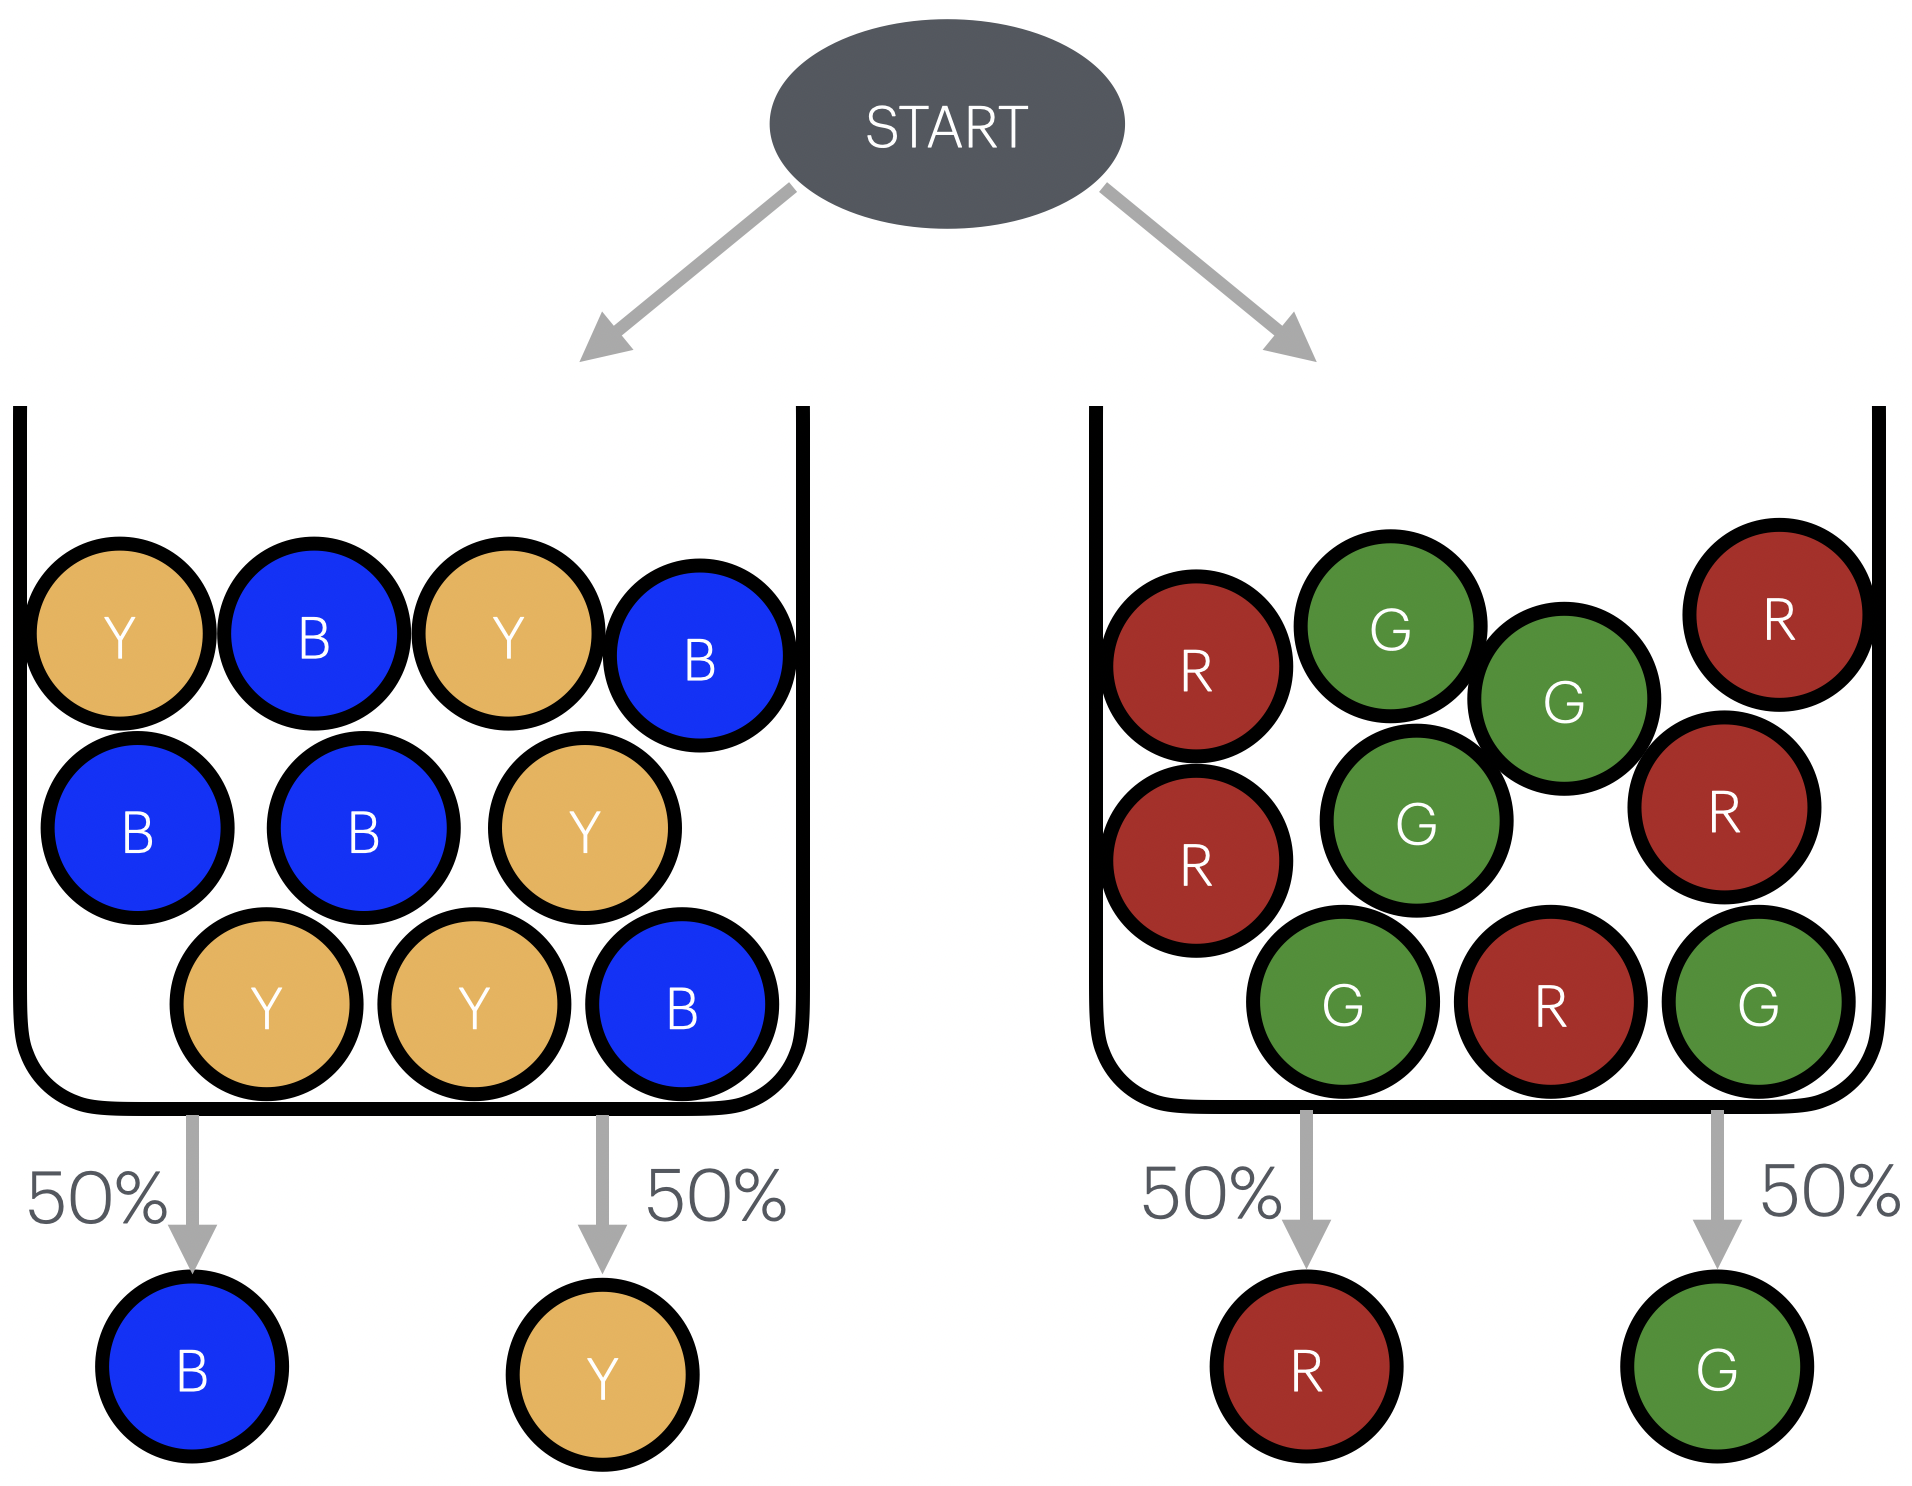
\includegraphics[height=4cm]{01-experiments/01-exp-descrNormInference/public/images/marble-machine.png}
\caption{The marble machine has two compartments, and one marble is released from each when the user presses the `start' button.}
\label{fig:sub1}
\end{subfigure}%
\begin{subfigure}{.5\textwidth}
\centering
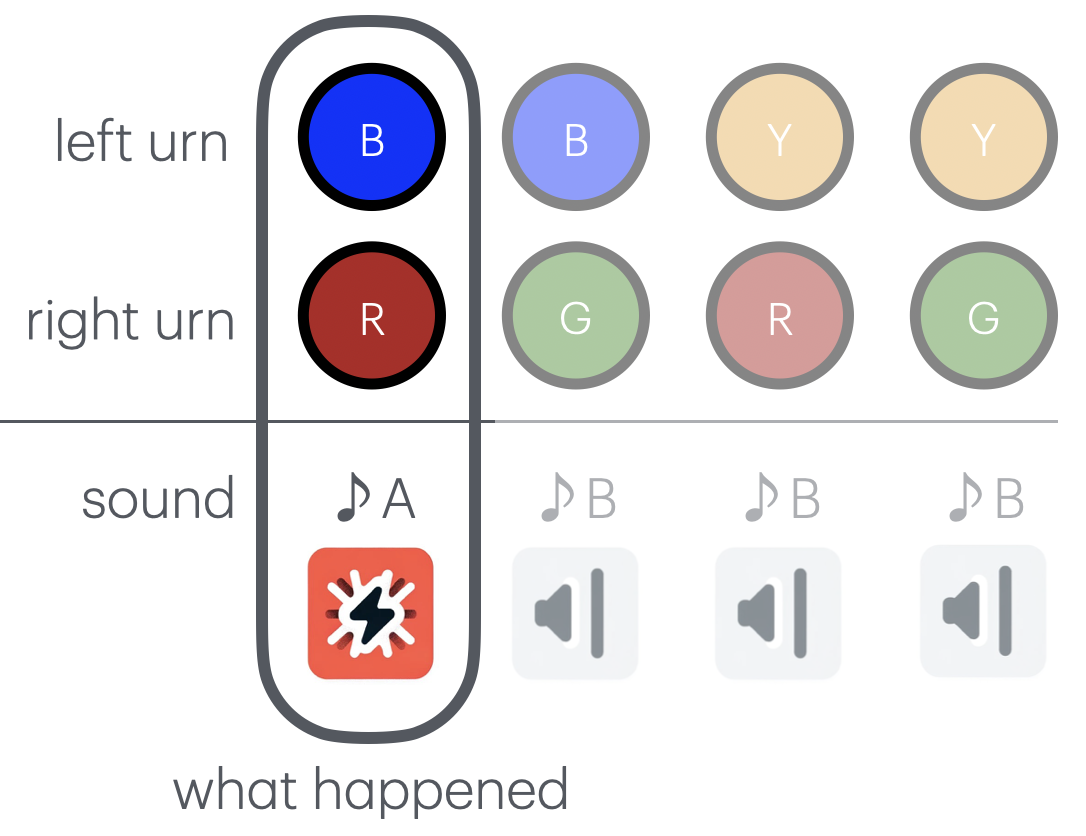
\includegraphics[height=4cm]{01-experiments/01-exp-descrNormInference/public/images/final-outcome-conjunctive-unpleasant.png}
\caption{Participants see what happened, as well as counterfactual outcomes for the other possible combinations of colors. This picture shows the negative valence, conjunctive condition.}
\label{fig:sub2}
\end{subfigure}
\caption{Illustration of the procedure, Study 1 (using pictures shown to participants).}
\label{fig:methods}
\end{figure*}

We also tell participants that there are two main religions on the island. Followers of Religion 1 think that Red is a morally bad color, while followers of Religion 2 think that Blue is a morally bad color. So, when islanders use the machine, they think (depending on their religion), that red marbles should not be released, or that blue marbles should not be released. Importantly however, instructions make it clear that i) users have no control over which color is released when someone uses the machine, ii) islanders from different religions agree on how the marble machine works.

We then told participants that an islander had used the machine, and a blue marble as well as a red marble were released, therefore sound A played. The islander said `The machine emitted sound A because a [red / blue] marble was released' (we randomized which color was mentioned). Participants were not told the islander's religion. They were asked to rate whether the islander is more likely to think that red marbles or blue marbles shouldn't be released, on a Likert scale from 1 (red marbles) to 7 (blue marbles), where 4 represents total uncertainty.

Participants then completed a short series of optional demographic questions, and were taken to Prolific for payment. The experiment also featured the following comprehension questions. After we described how the machine worked, we probed whether participants understood the causal structure: We showed them the four different possible combinations of marble colors released from the two compartments, and asked them which sound would be played in each case (each question was presented on a separate screen, and a reminder of the rule was displayed on top of the screen). We also asked participants who on the island knows how the machine works (\textbf{everyone} / followers of religion 1 / followers of religion 2), and whether a user who activates the machine can control which color gets released (true / \textbf{false}). We excluded from analysis participants who failed at least one comprehension question.

The experiment was implemented on a web interface built using Magpie (Franke et al., 2021). Interested readers can take the study at this \href{https://magpie-ea.github.io/magpie3-inferences-from-causal-attribution/}{\color{blue}{link}}. Data and R code for analysis are available on \href{https://github.com/magpie-ea/magpie3-inferences-from-causal-attribution}{\color{blue}{Github}}.\\


\subsubsection{Participants}
We recruited 305 participants from Prolific [ADD DETAILS IF RELEVANT]. We excluded from analysis participants who failed at least one comprehension question, for a final sample of 241 participants.

\subsection{Results}

Figure \ref{fig:resultsStudy1} displays the results. An analysis of variance revealed a main effect of outcome valence, F(2, 238) = 40.1, p < .001, a main effect of structure, F(1, 238) = 5.4, p = .02, as well as an interaction between structure and outcome valence, F(2, 238) = 3.34, p =. 04.

Follow-up Tukey HSD tests revealed the following patterns. Participants were more likely to infer that the cause is norm-violating in the unpleasant condition compared to the neutral and pleasant condition, p < .001. Participants were also more likely to infer that the cause is norm-violating in the neutral compared to the pleasant condition, p = .001.

Causal structure only had a significant effect in the neutral condition, where participants in the conjunctive condition gave higher ratings than in the disjunctive condition, p = .04 (corrected for multiple comparisons). Ratings did not differ by causal structure in the unpleasant condition, p = .98, or in the pleasant condition, p = .98.

Next we tested whether ratings in a given condition were significantly different from the midpoint of the scale (4). Ratings in the unpleasant condition were significantly higher than 4, M = 5.82, t(77) = 9.6, p < .001; while ratings in the pleasant condition were significantly lower than 4, M = 3.13, t(81) = -3.86, p < .001. In the neutral valence condition, ratings in the conjunctive structure were significantly higher than 4, M = 4.82, t(38)=2.52, p =.02, while ratings in the disjunctive structure were non-significantly lower than 4, M = 3.6, t(44) = -1.49, p = .14.





\begin{figure}[ht]
\begin{center}
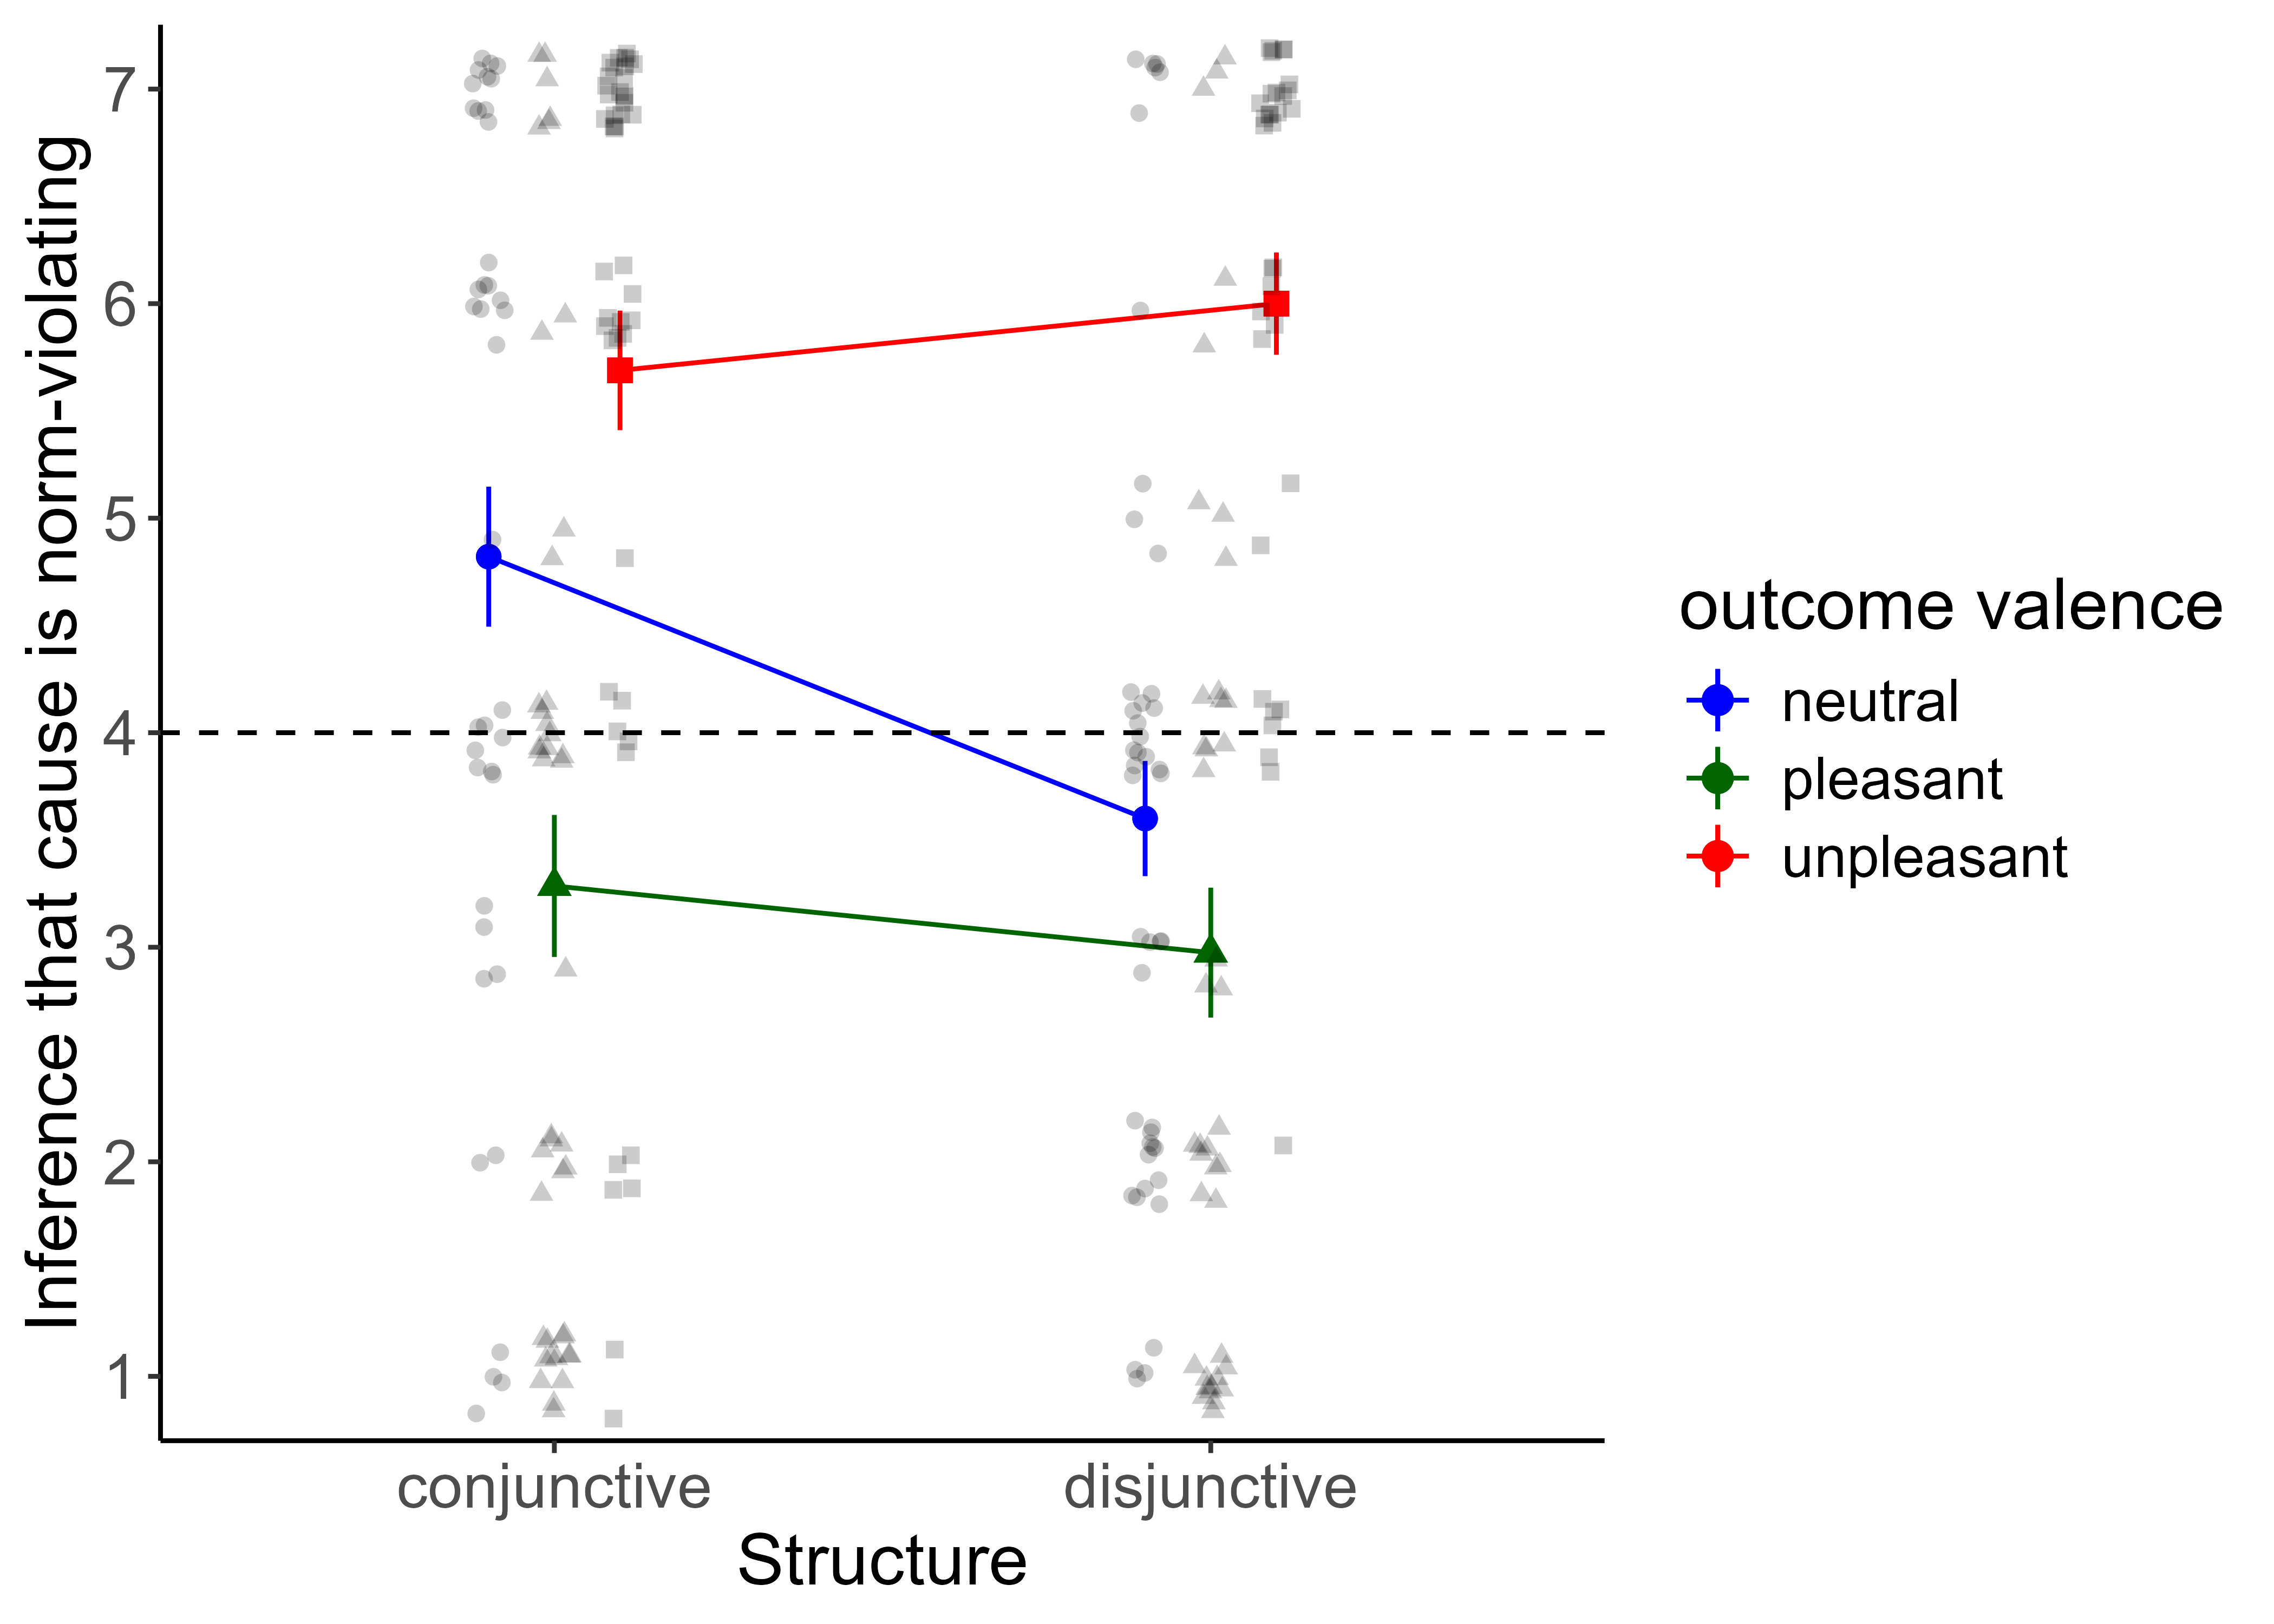
\includegraphics[scale=.5]{ResultsStudy1.png}
\end{center}
\caption{Results, Study 1. Error bars represent standard errors.}
\label{fig:resultsStudy1}
\end{figure}


\subsection{Discussion}
We find that listeners make systematic inferences about the prescriptive norm held by a speaker when they hear a causal judgment. Furthermore, we find that these inferences have a complex pattern.

When the outcome has a neutral valence, listeners' inferences depend on the causal structure. They infer that the cause violates a prescriptive norm in a conjunctive, but not a disjunctive causal structure. This pattern is what one expects if listeners were `reverse-engineering' the counterfactual simulation process underlying the speaker's causal judgment. This result provides a conceptual replication of the prescriptive norm inference result in Kirfel et al. (2022), while controlling for statistical normality, and showing that listeners make the inference even when they did not previously make causal judgments themselves.

In addition, we find that the valence of the outcome has a large effect on listeners' inferences. Listeners had a strong tendency to infer that the cause violated a norm when the outcome was bad, while they had a slight tendency to make the reverse inference when the outcome was good. Interestingly, there was no evidence for an effect of structure on listener's inferences when the outcome was good or bad. This contrasts with the results in the neutral condition. 

This latter result suggests a possible limitation in listeners' ability to reverse-engineer the causal judgment process. In studies of causal judgment, manipulating the causal structure typically has an effect on causal judgment even when the outcome has non-neutral valence \citep{kominsky2015causal, icard2017normality}. Furthermore, while outcome valence has an effect, that effect is typically smaller than the effect of norm violation \citep{alicke2011causation, kominsky2015causal, icard2017normality}. Perhaps the idea that people blame bad outcomes on things they don't like is so intuitive that listeners over-rely on that idea, neglecting to engage in more complex inferences.

\printbibliography[heading=bibintoc]

\end{document}
